\documentclass[12pt]{article}

\usepackage{fullpage}
\usepackage{graphicx, rotating, booktabs} 
\usepackage{times} 
\usepackage{natbib} 
\usepackage{indentfirst} 
\usepackage{setspace}
\usepackage{grffile} 
\usepackage{hyperref}
\usepackage{adjustbox}
\usepackage{amsmath}
\usepackage{siunitx}
\usepackage{multirow}
\setcitestyle{aysep{}}


\singlespace
\title{\textbf{Public Attitudes Towards Military Alliances}}
\author{Joshua Alley \\
Postdoctoral Research Associate \\
University of Virginia.\thanks{Thanks to Erik Lin-Greenberg, Todd Sechser, and Justin Schon, as well as participants in the Democratic Statecraft Lab Research incubator, the Lansing B. Lee/Bankard Seminar in Global Politics, 2020 Annual Meeting of the Peace Science Society and 2021 Meeting of the International Studies Association for helpful comments.} \\
jkalley@virginia.edu
}
\date{\today}

\bibliographystyle{apsr}

\begin{document}

\maketitle 

\doublespace 

\begin{abstract}
Why do Americans support or oppose military alliances? 
Although public backing for promises to defend other countries shapes the credibility and durability of U.S. alliance commitments, we know little about the foundations of public opinion towards alliances.
In particular, existing survey evidence cannot determine whether alliance attitudes are the top-down result of elite cues, or a bottom-up function of individual concerns and perceptions of alliance obligations and partners. 
In this article, I identify three determinants of public opinion towards alliances: elite cues, individual considerations, and alliance characteristics. 
I then use two conjoint survey experiments to assess the relative importance of these factors for public attitudes towards forming or maintaining international alliances.  
I find that ... 
\end{abstract}


\newpage 


\section{Introduction}

% lay out the question
What determines U.S. public opinion towards military alliances? 
Despite the importance of public attitudes for forming and upholding U.S. alliances, we do not know why the public supports or opposes alliance commitments. 
Opinion polls measuring public sentiment towards salient alliances like the North Atlantic Treaty Organization (NATO) can describe aggregate support and show changes over time, but they do not explain why individuals express particular alliance attitudes. 


% Three explanations to adjudicate between/compare
In this article, I consider three explanations of public attitudes towards alliances; individual concerns, elite cues, and alliance characteristics.
The relative importance of these three factors has implications for a broad debate about whether public foreign policy attitudes are bottom-up or top-down. 
First, individual concerns such as partisanship, foreign policy dispositions, and economic interests shape public foreign policy attitudes \citep{KertzerZeitzoff2017}.
Alliance characteristics such as military capability, economic ties, regime type, common threat, or treaty obligations could also mold individual assessments of alliances, especially by appealing to particular individual concerns. 
If individual concerns and alliance characteristics are the key drivers of alliance opinions, then public attitudes reflect a bottom-up process. 
On the other hand, if public sentiment towards alliances responds primarily to elite cues, alliance attitudes permeate from the top down.
If partisanship has the dominant influence by shaping receptiveness to elite cues and alliance characteristics, alliance attitudes mix top-down and bottom-up elements as individuals integrate information from multiple sources \citep{PageShapiro1992}.  


% Importance part 1: public opinion undergirds alliance com in democ
There are three reasons that understanding U.S. public opinion towards alliances is worthwhile. 
To start, public support plays a key role in debates over how democracies make reliable promises of military support. 
If public opinion towards alliances is driven by individual concerns and alliance characteristics, this may lead to relatively stable public opinion and reliable commitments \citep{Gaubatz1996}.
If elite cues are more consequential, then alliance opponents could quickly shift public opinion and generate a cycles that hinder democratic reliability \citep{GartzkeGleditsch2004}.
Public opinion also affects the political sustainability of alliance commitments.\footnote{Public opinion is important, but it is not deterministic. \citet{Kreps2010} notes that public disapproval may not hinder coalition warfare in formal multilateral alliances, especially when elite consensus favors fighting.}
For example, NATO leaders often feared that changing public attitudes would undermine the alliance \citep{Sayle2019}.   


% importance part 2: practical relevance- US role in world. 
Why the public supports or opposes alliances also speaks to the practical consequences of a prominent debate in U.S. foreign policy. 
Two competing visions of future U.S. foreign policy depend heavily on alliances. 
One view believes that the United States should reduce its alliance commitments as part of a more restrained grand strategy \citep{Preble2009, Posen2014}.
The other argues that continued deep engagement through alliances is the best way to promote U.S. security and prosperity \citep{Brooksetal2013, BrandsFeaver2017}. 
If elite cues drive public opinion, policymakers and political leaders have substantial latitude to change U.S. alliance commitments. 
But if public opinion towards alliances is based on individual intuitions and alliance characteristics, elites risk public disapproval if they undermine popular alliances.  
For example, some observers feared that Donald Trump's criticism of U.S. alliances would weaken domestic support for alliances.
Yet public approval of alliances like NATO remained steady in the United States during the Trump administration \citep{PewNATO2020}. 


% importance part 3: WHY support international cooperation, not just consequences of international institutions
In addition to its practical importance, this study fills a gap in international institutions scholarship. 
Scholars are more likely to study how international institutions affect public attitudes (e.g. \citep{KayaWalker2014, Greenhill2020}), than scrutinize the sources of public attitudes towards international institutions themselves. 
Other studies use observational survey data to examine public opinion towards international cooperation such as multilateral financial institutions \citep{Edwards2009} or the United Nations \citep{Torgler2008, DellmuthTallberg2015}. 
There is little experimental evidence of why the public supports or opposes alliances.
In one study of public opinion and military alliances, \citet{TomzWeeks2021} show that the presence of an alliance increases public support for foreign military intervention. 
\citet{Chuetal2021} explore how values and interest based elite cues shape public attitudes towards alliance maintenance. 
I build on these works with a more general experiment on alliance attitudes that spans elite cues, alliance characteristics and individual factors. 


% survey on NATO, etc don't get at it
There is therefore little evidence to explain why individuals support forming and maintaining military alliances. 
Tracking changes in public opinion over time in standard surveys gives useful descriptive data on alliance maintenance, but it  does not provide causal evidence.
For example, surveys of NATO measure public support, but they cannot say whether it is the result of cooperative individual dispositions, backing an alliance with other democracies, or elite support. 
This study disentangles the three mechanisms by simultaneously assessing the impact of all three on attitudes towards alliance formation and maintenance. 


% Assess w/ a survey experiment
I use two conjoint survey experiments to assess the relative influence of individual concerns, elite cues and alliance characteristics on public opinion towards alliances. 
Conjoint experiments randomize multiple alliance characteristics and elite cues, so this tool is well-suited to assessing the relative weight of different factors \citep{Hainmuelleretal2014}.
The first study asks individuals to rate five hypothetical new alliance commitments and support or oppose alliance formation.
The second asks respondents to rate five hypothetical existing commitments and support or oppose alliance maintenance. 
Both studies start by measuring individual foreign policy dispositions, ideology, and economic interests. 
I then follow this with the five choice and rating tasks for hypothetical alliances. 
This analysis allows me to estimate the relative weight of the three mechanisms while assessing whether public opinion differs across alliance formation and maintenance.  


% findings
In two nationally representative survey experiments, I find that...


% Implications
The results imply that. 


% Try it w/o the plan of paper for flow. 


\section{Three Explanations of Public Opinion Towards Alliances}

Public opinion is a critical part of democratic foreign policy and alliance politics.
Public approval guides decisions about military force and whether to intervene in foreign conflicts \citep{Tomzetal2020, LinGreenberg2021}. 
In democracies, anticipation of public disapproval of treaty violation encourages conditional promises of military support \citep{Chibaetal2015, FjelstulReiter2019}. 
Moreover, public attitudes have a key role in disputes about the reliability of democratic alliances \citep{Gaubatz1996, GartzkeGleditsch2004}. 
Last, policymakers pay careful attention to public support for alliances \citep{Sayle2019}. 


% NATO example to bring out the puzzle
There is also meaningful variation in pubic opinion towards military alliances. 
\autoref{fig:nato-op-time} plots the percentage of respondents supporting NATO in 59 surveys from 1974 to 2020.\footnote{These surveys ask respondents to assess NATO in many ways. I consider favorable opinions, feeling thermometer ratings of 50 or higher, and support for increasing or maintaining U.S. commitment as indicators of support for NATO.} 
NATO generally commands majority support in public opinion, but average support has fallen since 2000. 
Although the general public opinion patterns are clear, this does not explain why individuals support alliances and why support changes over time. 


\begin{figure}
	\centering
		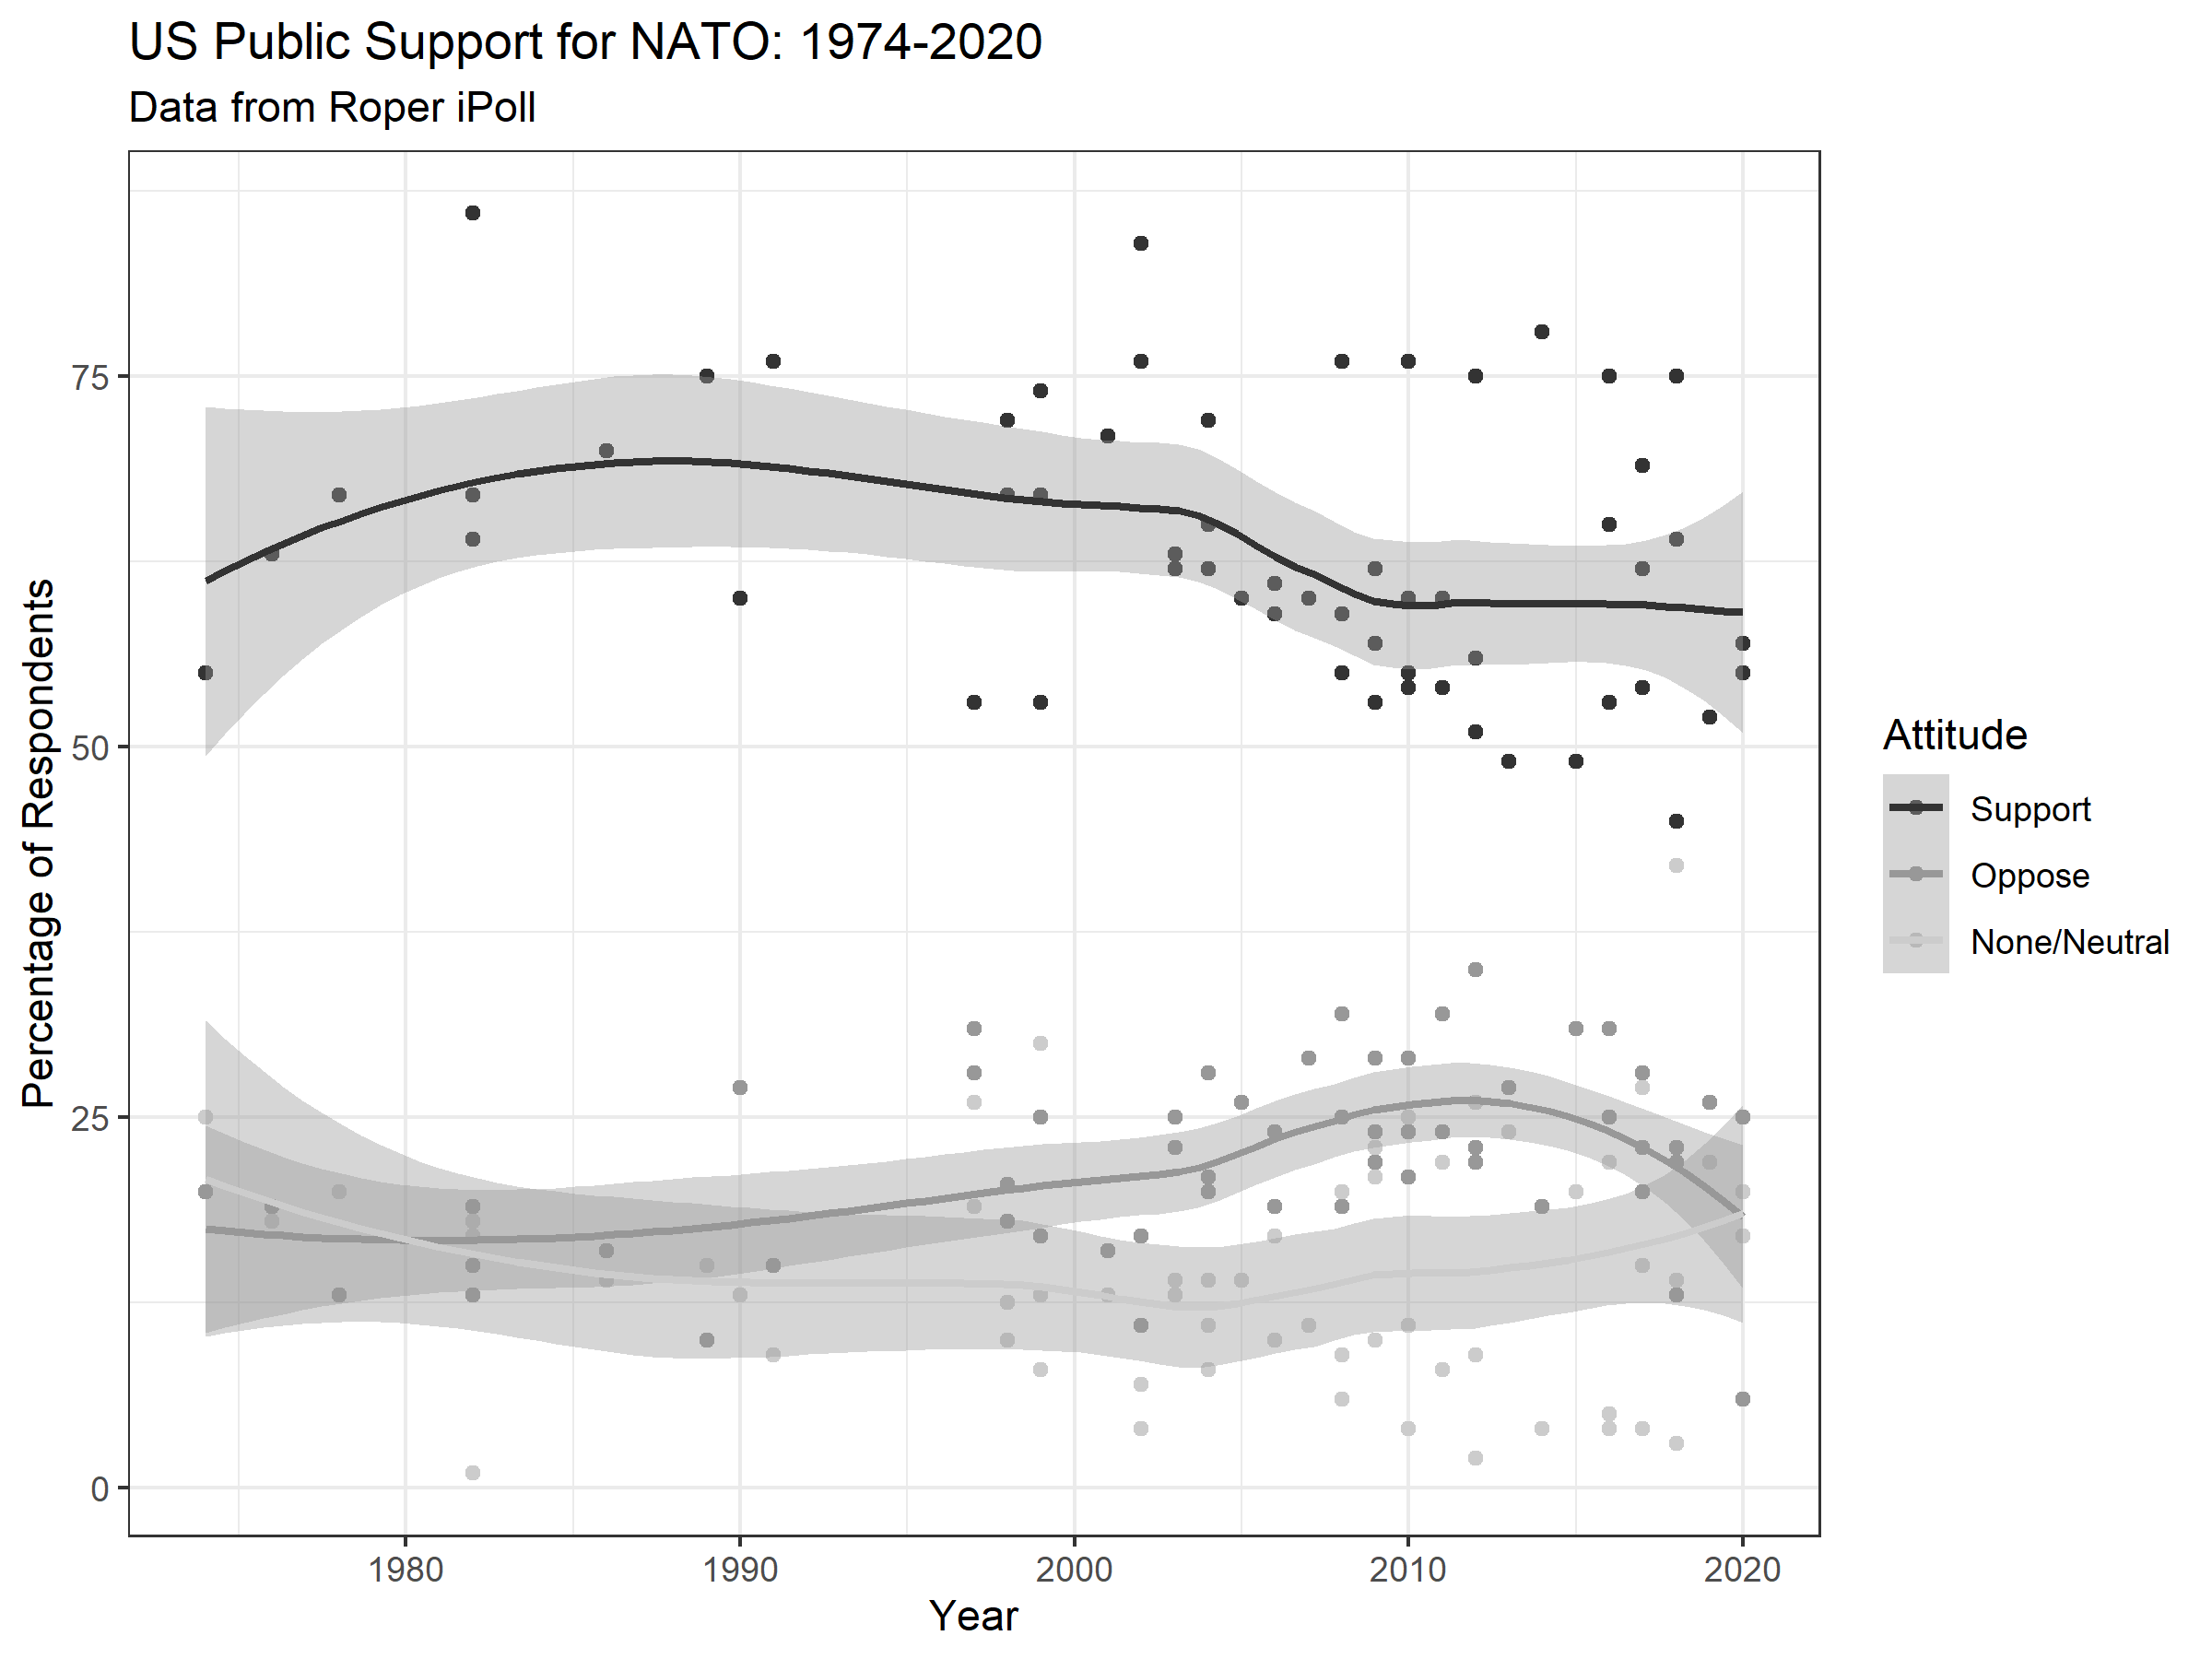
\includegraphics[width=0.95\textwidth]{../figures/nato-op-time.png}
	\caption{US public support for NATO from 1974 to 2020. Each point marks a unique poll, and colors differentiate the percentages of respondents that expressed support, opposition or neutral/no opinion of NATO. Loess lines estimate the average support for each group in every year. Topline data from the Roper Center's iPoll database.}
	\label{fig:nato-op-time}
\end{figure}


Individual foreign policy dispositions, elite cues, and alliance characteristics are all plausible explanations of alliance attitudes.
This is turn generates a puzzle--- are public attitudes towards alliances a top-down result of elite cues or a bottom-up function of individual concerns and alliance characteristics? 
On the one hand, limited public information about alliances could give elite cues and framing substantial influence \citep{Druckman2001}. 
On the other, the public opinion towards alliances may depend more on individual dispositions and intuitions about international affairs \citep{KertzerZeitzoff2017} and material interests \citep{RhoTomz2017}.
A strong role for individual assessments of alliance characteristics implies a bottom up process, as the public uses information about an alliance to form a considered opinion instead of depending on elite cues.
If individual concerns are highly influential, they will alter the appeal of specific alliance characteristics. 
For example, as I detail below, individuals with greater international economic ties might be more likely to support alliances with trade partners.  


Alliance characteristics could also shape elite cues, but the implications for public opinion are unclear. 
Foreign policy elites such as elected officials, military leaders and diplomats have diverse ideological, institutional and practical concerns. 
Particular elites can thus justify or criticize alliance commitments for different reasons, which makes predicting elite cues for specific alliance profiles difficult. 
Regardless, an elite leading model implies that no matter how elites arrived at their judgment, public attitudes will follow their cues. 
If individuals discount elite cues and pay more attention to whether specific alliances are worthwhile, that implies a more bottom up process. 


The relative importance of the three mechanisms for public opinion towards international alliances thus speaks to fundamental debates about the sources of public opinion on foreign policy issues.  
In the following, I explain each mechanism in greater detail. 
I also consider how each factor would explain changes in public attitudes towards alliances over time. 


\subsection{Individual Concerns}
% Kertzer stuff- bottom up, some individuals are more cooperative in general
% also about threat/need


% Overview para
Individual considerations are one determinant of public attitudes towards alliances. 
Potential individual sources of alliance opinions include foreign policy dispositions, material interests and partisanship. 
These factors shape perceptions of the costs, benefits and value of international cooperation. 
As such, the impact of individual concerns will be reflected in divergent perceptions of alliance obligation and benefits that depend on foreign policy disposition, economic interests and partisanship. 
Put differently, individual concerns will usually shift alliance attitudes by altering the salience of different alliance characteristics. 


% foreign policy disposition
Many individuals have stable intuitions about the best way to approach international politics. 
Militant assertiveness and internationalism \citep{Herrmannetal1999} are two such foreign policy dispositions.  
These principles shape how individuals respond to foreign policy decisions, such as backing down from promises of military intervention \citep{KertzerBrutger2016}. 


% internationalists more likely
% Define internationalism  
Internationalism reflects an inclination to work with other countries and contribute to international institutions. 
Internationalist respondents generally support American engagement in foreign affairs and will likely favor alliance commitments. 
Conversely, isolationist respondents are more skeptical of international institutions and cooperation. 
Isolationists distrust foreign involvement and often advocate for more emphasis on domestic affairs. 
As a result, isolationists will be generally skeptical of alliances, and especially opposed to alliances with broad support conditions or deep cooperation. 


% militant assertiveness 
The relationship between militant assertiveness and alliances is less obvious. 
Hawkish individuals are more willing to use force to address international problems. 
Although alliances are a cooperative institution, they also aggregate military capability \citep{FordhamPoast2014}. 
Hawkish respondents may worry that alliance commitments drain U.S. strength, or support capability aggregation through alliance commitments. 


% material interests- trade/investment
In addition to foreign policy dispositions, individuals may have material interests in backing international alliances.
Military alliances promote economic ties between members, including trade \citep{Gowa1995, LongLeeds2006}, foreign investment \citep{LiVashchilko2010} and currency pegs \citep{Li2003}. 
Just as individuals who benefit from international commerce back trade liberalization \citep{RhoTomz2017}, individuals with internationally-oriented occupations and economic interests could support alliances that bolster international commerce or protect trade partners. 
On the other hand, individuals who lose out from lost trade protection under an alliance \citep{WolfordKim2017} are more likely to oppose alliances.


% partisanship 
Partisanship subsumes some foreign dispositions and material interests. 
Republicans and conservatives in the United States have a longstanding history of isolationist sentiment, for instance \citep{Kupchan2020}.
As a result, they are usually more skeptical of international engagements like alliances. 
Republicans also tend to be more hawkish. 
Partisanship may thus encompass the key foreign policy dispositions and dominate individual alliance attitudes. 


Party identification also mixes elite cues and individual concerns, as it may amplify the influence of some elite cues and diminish the impact of others.
Individuals may largely respond to cues from co-partisan elites, for example. 
Given its capacity to subsume some foreign policy dispositions and shape receptiveness to elite cues, partisanship may be especially influential. 


% change over time: generations
These individual concerns could explain changes in public support for alliances over time through generational shifts and changing economic opportunities. 
As the experiences of each generation mold their foreign policy dispositions, public opinion of alliances will slowly shift over time. 
Changes in economic opportunities, including trade shocks from alliances, could also change alliance attitudes. 
These mechanisms imply that the public opinion towards alliance commitments will usually change gradually. 



\subsection{Alliance Characteristics}
% some alliances are more attractive than others
% look to other results- democ, strength, etc. 
% economic interests

Alliance characteristics are the second potential determinant of public opinion towards alliances.
Military alliances take many forms, as states negotiate distinct treaties with diverse partners.
Allied capability, shared interests, and the nature of the alliance obligations are all plausible determinants of alliance attitudes.   
When individuals form an opinion about an alliance, these alliance characteristics are another possible influence. 
Rather than look to elite cues, the public may weigh the specific merits of each alliance, especially based on their individual concerns. 


% describe top-down/bottom up connection here 
Limited public information on foreign policy issues may constrain the impact of alliance characteristics, however. 
Especially if the public relies on elite cues, individual intuitions about the worth of a specific alliance commitment will be weak. 
But if alliance characteristics shape public opinion more than elite cues, this would increase the stability of public opinion towards international alliances and constrain elite alliance formation and maintenance. 


% Capability
Allied capability is the first major alliance characteristic.
Greater allied capability should generally increase the appeal of an alliance. 
All else equal, alliances with militarily capable states are more valuable \citep{Johnsonetal2015}. 
Inasmuch as the public understands that allies with substantial military capability have greater capacity to deter and fight, they will back alliances with more capable states. 


\subsubsection*{Shared Interests}

% Shared interests
Perceptions of shared interests with allies are another salient alliance characteristic. 
Common threat, economic ties, democratic political institutions and recent military operations are all observable indicators of common interests. 
Public perceptions of a shared threat may be especially important. 
Alliance treaties make costly promises to intervene in military conflicts. 
The public may only be willing to hazard the costs of intervention under serious threat. 
If individuals do not believe that the alliance addresses a security threat, they will be less likely to support protecting foreign states. 


% Economic ties
Economic ties are another indicator of shared interests. 
Protecting trade ties often motivates asymmetric alliances between large and small states \citep{Fordham2010}. 
As individuals value foreign trade and investment and see it as an indicator of common interests, they will approve of alliance commitments with trade partners.
Individual economic interests likely modify the salience of trade ties, however.


% Democracy 
Democratic citizens may also prefer alliances with other democracies. 
At a minimum, the democratic public rarely supports military strikes against other democracies \citep{TomzWeeks2013}. 
Individuals may believe that democracies should cooperate because they share common concerns and values. 
Values are a plausible justification of alliance participation \citep{Chuetal2021}. 
Domestic political regimes thus offer a simple heuristic for a trustworthy and valuable alliance partner. 


% Recent conflict participation
Recent military operations are the final salient indicator of shared interests. 
If the United States and a potential alliance partner or current ally recently participated in a common military operation, the public could believe that they share common concerns and interests. 
Recent military operations would also suggest that the other state will bear substantial costs to support the United States. 
This applies to both alliance formation and maintenance. 
For example, U.S. allies participated in operations in Iraq and Afghanistan, but so did states such as Georgia and Ukraine who did not have a formal defense treaty.\footnote{Some states may have participated in wartime coalitions to seek closer alignment with the United States \citep{GannonKent2020}.}


% shared interests and cap as key explanations of changes over time. 
Indicators of shared interests and changes in allied capability could explain temporal variation in alliance attitudes. 
Threat perceptions and recent military operations are both salient contextual factors. 
If public perceptions of common interests wane, support for alliances will fall. 
For example, reduced allied capability could create beliefs that partners are not pulling their weight or contributing enough capability. 
Democratic backsliding might also lead the public to question whether allies share U.S. interests and values. 



\subsubsection*{Alliance Obligations}


% Alliance treaty design 
In addition to shared interests, the nature of the alliance obligations may shape public support for alliances, especially alliance formation. 
There is immense variation in alliance treaty content \citep{Leedsetal2002}.
Potential alliance members must agree on whether they are willing to offer military support, conditions on that support, and how they will contribute to deterrence and/or war fighting \citep{Poast2019a}. 
These issues are reflected in alliance treaties, which stipulate military intervention, conditions on allied support, defense cooperation, and issue linkages, all of which could impact alliance attitudes. 


% conditionality
Half of all defensive alliances restrict promises of military support to particular circumstances such as non-provocation, certain locations, or specific adversaries. 
These promises reduce the risk of entrapment \citep{Benson2012}, as unconditional support exposes states to violating the treaty or supporting an ally in unwanted conflicts.
If the public fears entrapment in foreign conflicts or reckless allies, they will prefer alliances with conditional obligations.\footnote{\citep{Chibaetal2015} find that democracies are more likely to design alliances with conditional promises of military support, and they attribute this to elite attempts to make alliance commitments they are able to fulfill. Public disapproval of unconditional support could also explain this relationship, however.}
Most U.S. alliances restrict promises of intervention to attacks on allies and conflicts in specific regions. 


% Depth sources 
Other alliances supplement the core promises of military support with peacetime defense cooperation \citep{Morrow1994, LeedsAnac2005}. 
These treaties include basing rights, integrated military commands, military aid, formal organizations or other costly cooperation to coordinate policies and establish credible commitments.
Almost half of all military alliances have some defense cooperation \citep{Leedsetal2002}, and many U.S. alliances include formal organizations, bases, and military aid. 
The public may prefer more arms-length commitments, or back strong ties with allies. 


% financial costs
In addition to formal treaty obligations, military alliances increase U.S. defense spending \citep{AlleyFuhrmann2021}. 
While the public may accept the costs of alliances, alliance skeptics often highlight the financial costs of alliance commitments \citep{Posen2014}. 
Growing financial costs could easily reduce public support for alliance commitments, especially among Republicans and isolationists. 


% issue linkages
Last, formal and informal issue linkages often support credible alliance commitments \citep{Poast2013}. 
Connecting other issues like trade rights or economic aid to alliance negotiations can facilitate agreement \citep{Poast2012}.
With issue linkages, states make concessions in different areas to conclude a general agreement. 
Perceptions that an alliance brings further trade or foreign policy concessions could increase public approval.  


% obligations are less dynamic
Alliance obligations are less likely to explain changes in public opinion over time than individual dispositions or contextual factors like threat, trade and allied democracy. 
Fixed treaty obligation cannot explain variation in alliance attitudes over time. 
Treaty obligations could affect public support for treaty formation, however. 


Both alliance characteristics and individual considerations are bottom-up mechanisms of public opinion towards alliances. 
In these frameworks, individual characteristics and intuitions drive support for alliances and may constrain elite policies. 
A bottom up framework can also explain cross-sectional support and changes in support over time, either through generational change or shifting circumstances. 
Elite cues offer another explanation for public attitudes, however. 



\subsection{Elite Cues} 
% Framing/elite leading
% Debate over leading/pandering

Although the confluence of individual concerns and alliance characteristics is a plausible explanation of alliance attitudes, elite cues are equally plausible. 
The public often relies on co-partisan elites for guidance \citep{Druckmanetal2013}. 
In this case, elite portrayals of alliances bolster or undermine public support for alliance commitments as the public follows the lead of trusted elites in forming their opinion. 
The elite cues framework implies that public opinion towards alliances is endogenous to elite views \citep{Druckman2014}.


If elite cues are the most important factor, public opinion towards alliances is largely a top-down phenomenon.
There is also substantial evidence that elites influence public foreign policy attitudes. 
The media inform the public, but they also convey elite frames \citep{BaumPotter2008} and social media may further amplify elite influence \citep{BaumPotter2019}.   


Furthermore, information shortcomings make individuals more responsive to elite framing and cues \citep{Druckman2001, Peterson2017}.  
The public has limited information about foreign policy relative to domestic issues, and alliance politics are not usually salient even within foreign policy. 
Therefore, elite support or opposition could have a profound influence on alliance attitudes as individuals rely on trusted elites. 


% cue-giver matters
Elected officials, diplomats and military leaders are all potentially influential in alliance politics. 
Cues from military leaders can shape public opinion about the use of force \citep{Golbyetal2018}, so military endorsements may be especially influential. 
Public perceptions that military leaders and diplomats are well-informed about alliances will likely increase their influence. 


Partisanship also shifts how elected leaders exert influence.
With extensive partisan polarization, individuals discount messages from out-partisan elites. 
Conversely, trust increases the influence of messages from copartisan elites. 
Support for alliances by co-partisan elites should increase individual support for alliances, and elite criticism would reduce public support.  
Unified elite cues would be especially influential by tapping support on both sides of partisan divides.
For example, \citet{Berinsky2007} finds that unified elite support for war also increases public support. 


% explanation over time
The elite cues model offers a different process for understanding changes in alliance attitudes over time. 
In this framework, shifting public attitudes reflect new elite cues. 
Conversely, stable public opinion would indicate consistent elite views. 


Elites, especially elected leaders, might pander to existing public attitudes, however.\footnote{See \href{https://fivethirtyeight.com/features/is-trump-fueling-republicans-concerns-about-nato-or-echoing-them/}{this article} for a discussion of pandering and leading in the case of Trump and NATO.}
Under a pandering framework, convergence between elite rhetoric and public opinion reflects elites conforming their support to public opinion, rather than shaping public attitudes. 
If elite rhetoric on alliances is mostly pandering to opinions that were derived from individual and alliance characteristics, then elite cues will have little effect on alliance opinions.


Evidence on whether elites pander to or lead public opinion is divided.
Some evidence suggests that elite pandering is rare. 
\citet{Canes-Wrone2006} finds that Presidents rarely pander to the public unless they already agree with public preferences.
\citet{Kreps2010} notes that public disapproval did not constrain participation in NATO's International Security Assistance Force in Afghanistan. 
Moreover, foreign policy is a secondary concern for many voters, so elite foreign policy views and rhetoric can diverge from public attitudes with few political repercussions \citep{BusbyMonten2012}. 


Other studies suggest that elites match their rhetoric to public opinion. 
\citet{Barberaetal2019} use social media data to show that legislators are more likely to follow than lead public opinion on issues. 
Similarly, \citet{HagerHilbig2020} find that exposure to public opinion research moves speech and policy positions by German positions closer to majority opinion. 
\citet{GuisingerSaunders2017} note than for issues with low partisan polarization, information effects can dominate public opinion, though elite cues matter more for polarized issues like cap and trade schemes. 
Even military elites may shape their recommendations in response to public opinion \citep{LinGreenberg2021}. 


Therefore, the top-down and bottom-up approaches are both plausible models of public opinion towards alliances. 
The public is unlikely to have substantial information about alliance politics, which should increase elite influence. 
At the same time, individual foreign policy dispositions are an influential factor in public opinion \citep{Herrmannetal2009, KertzerZeitzoff2017}, so intuitions about the value of alliances or salient alliance characteristics might be more influential. 


% drawing on multiple sources
It is also possible that alliance attitudes has both top-down and bottom-up elements. 
\citet{PageShapiro1992} note that public opinion is broadly consistent and rational, and changes in predictable ways in response to information from multiple sources, including elite cues. 
Partisanship is especially important in this respect. 


% partisanship mixes
If partisanship has a large role in shaping the impact of elite cues and alliance characteristics, then alliance attitudes mix top-down and bottom-up elements. 
Party identification is tied to both elite cues and individual concerns, as it makes individuals more receptive to specific elite cues and encompasses key material and ideological concerns. 
In the following data, Republicans are slightly higher on isolationism and military internationalism than Democrats or Independents, for instance. 
Partisans may therefore value different alliance characteristics. 


% allows 
The confluence of partisanship and foreign policy attitudes also creates some scope to explore how much elite rhetoric leads public opinion. 
If isolationist individuals are skeptical of alliances in general, they should be less responsive to cues from co-partisan elites.
But if elites can lead public opinion, elites cues will increase support for alliance participation even among isolationists. 


% formation vs maintenance
Before discussing how I examine the weight of individual concerns, alliance characteristics and elite cues, there are three important considerations. 
First, alliance formation and maintenance are distinct processes \citep{Snyder1997}. 
Forming a new alliance and upholding an existing commitment are subject to different considerations.
Therefore, I consider alliance formation and maintenance in separate survey experiments to assess whether the public views making a new alliance commitment and upholding an existing treaty differently. 


% interactions possible- especially between individual and alliance characteristics
Second, individual concerns, alliance characteristics and elite cues likely interact. 
Understanding how the impact of alliance attributes vary across partisanship, foreign policy dispositions, and economic interests is essential to assessing the impact of individual concerns. 
To give two examples, isolationists would express greater disapproval of unconditional alliances, while individuals with international economic ties should support treaties with substantial trade or economic issue linkages. 
Furthermore, Republicans and Democrats will more responsive to cues from co-partisan elected officials. 
In the analysis, I first estimate unconditional effects of elite cues and alliance characteristics, before analyzing differences in between partisan, economic, and isolationist and militant internationalist subgroups. 
The subgroup analyses provide crucial evidence on the role of individual concerns. 


% long-run cycles
Finally, feedback between elite cues and public opinion is plausible in the long run. 
It is possible that public opinion shapes elite cues, which in turn alter public opinion. 
For example, elites could respond to growing public opposition to an alliance by pandering and adopting more skeptical rhetoric. 
Elites could also attempt to lead public opinion and restore alliance support, however.
Such feedback would take time, and would be most obvious in the context of longstanding alliances.
For such a cycle to exist, elite cues must influence public alliance attitudes, however.
This analysis can therefore establish part of a potential feedback cycle. 
I now describe how I assess the importance of elite cues relative to individual concerns and alliance characteristics. 



\section{Experimental Design}


% justify conjoint: 
I use two conjoint survey experiments to assess how individual considerations, alliance characteristics, and elite cues shape public support for forming and maintaining alliances in the United States. 
As with many political phenomena, multiple alliance attributes could affect individual attitudes. 
Alliances bundle elite support and characteristics like threat and treaty obligations, each of which is a potential experimental treatment.  
Conjoint experiments allow researchers to decompose composite phenomena to estimate and compare the impact of multidimensional treatments \citep{Hainmuelleretal2014}. 
For example, \citet{HainmuellerHopkins2015} use a conjoint experiment to identify what types of immigrants Americans favor. 
\citet{BechtelScheve2013} assess how institutional design affects public approval for climate cooperation agreements with a conjoint experiment in four countries. 


% describe rating tasks
Both conjoint experiments ask individuals whether they support participation in a defensive alliance that has a randomly generated profile of alliance characteristics and elite cues. 
In the alliance formation experiment, I ask respondents to assess five hypothetical new alliances. 
In the alliance maintenance experiment, respondents rate five hypothetical existing alliance commitments.


Before presenting the alliance rating tasks, I measure key respondent characteristics, especially economic interests, political ideology, and foreign policy disposition.  
These measures provide the basis of the subgroup analyses examining how individual concerns shape alliance attitudes. 
The subgroup analyses assess whether support for alliance participation differs across groups as well as variation in the impact of different cues and alliance characteristics.


After measuring key individual factors, I present respondents with a table of information about a hypothetical alliance with a randomly generated profile of elite cues and characteristics.
Once respondents read the table, I then ask them to rate the alliance on a scale from 0 to 100 and express approval of alliance formation or maintenance with a yes/no question. 
I will then present four more randomly generated alliance profiles, so each respondent rates five hypothetical alliances in a single-profile conjoint design.\footnote{A two profile design would ask respondents to choose between two alliances, each with a random set of characteristics.} 


% Add a table with conjoint attributes. 
Each alliance partner profile is randomly generated from the attributes in \autoref{tab:conjoint-vars}.
Every attribute has multiple potential values and I produce the full alliance profile by randomly selecting one value from each attribute. 
I chose the set of attributes and values to capture theoretically interesting alliance characteristics and generate plausible profiles.\footnote{There are no restrictions on value combinations in the alliance profiles and I employ this uniform randomization because all of these alliance profiles are plausible.} % De la cuesta et al discussion here as needed
I randomize the order of the attributes in the table at the respondent level, so the order is the same for each respondent. 
Drawing alliance profiles at random and providing multiple rating tasks in a conjoint experiment makes estimating the average marginal component effect (AMCE) for each alliance attribute straightforward \citep{Hainmuelleretal2014}. 


\begin{table}
\begin{adjustbox}{width = .99\textwidth}
\begin{tabular}{lc} 
\hline \\ 
\textbf{Attributes} & \textbf{Values} \\
\hline \\ 
Republican Senators & Support an alliance with this country. \\
                    & Oppose an alliance with this country. \\ 
                    
Democratic Senators & Support an alliance with this country. \\
                    & Oppose an alliance with this country. \\ 
                    
The Joint Chiefs of Staff & Support an alliance with this country. \\
                    & Oppose an alliance with this country. \\ 
                    
The Secretary of State & Supports an alliance with this country. \\
                    & Opposes an alliance with this country. \\ 
                    
Trade Ties          & The United States has minimal trade ties with this country. \\
                    & The United States has modest trade ties with this country. \\
                    & The United states has extensive trade ties with this country. \\ 
% modified from Tomz and Weeks 2013 APSR: https://web.stanford.edu/~tomz/pubs/TomzWeeks-2013-11-Appendix.pdf 
Partner Political Regime    & This country is not a democracy, and shows no sign of becoming a democracy. \\
                    & This country is a democracy, but shows signs that it may not remain a democracy. \\ % democ backsliding
                    & This country is a democracy, and shows every sign that it will remain a democracy. \\
                    
Partner Military Capability & 10,000 soldiers and spends 1\% of their GDP on the military. \\ % low
                    & 80,000 soldiers and spends 2\% of their GDP on the military. \\ % moderate
                    & 250,000 soldiers and spends 3\% of their GDP on the military. \\ % high 
                    
Shared Threat       & The United States and this country face minimal common threats. \\ 
                    & The United States and this country face modest common threats. \\
                    & The United States and this country face serious common threats. \\
                    
Recent Military Cooperation  & This country has not participated in recent U.S. military operations. \\ 
                    & This country recently supported U.S. airstrikes against terrorists. \\
                    & This country recently supported U.S. counterinsurgency operations. \\
                    & This country recently fought with the United States in a war. \\
                    
Financial Cost      & This alliance requires \$5 billion in annual U.S. defense spending.  \\ 
                    & This alliance requires \$10 billion in annual U.S. defense spending.  \\ 
                    & This alliance requires \$15 billion in annual U.S. defense spending.  \\ 
                    
Conditions on Support  & The alliance treaty promises military support in any conflict. \\ 
                    & The alliance treaty promises military support only if this country did not provoke the conflict. \\ 
                    & The alliance treaty promises military support only if the conflict takes place in this country's region. \\
                    
Defense Cooperation & None. \\ 
                    & The alliance treaty provides basing rights for U.S. troops. \\
                    & The alliance treaty includes a shared military command. \\
                    & The alliance treaty includes an international organization to coordinate defense policies.  \\ 
% Issue linkages                    
Related Cooperation & None. \\
                    & The alliance is linked to greater trade and investment with the United States. \\ 
                    & The alliance is linked to greater support for the United States in the United Nations. \\ 
                    
Region              & Europe. \\ 
                    & Africa. \\
                    & The Middle East. \\ 
                    & Asia. \\   
                    & The Americas. \\ 
                                                                            
\hline \\
\end{tabular}
\end{adjustbox}
\caption{Table of alliance attributes in conjoint experiment profiles. I use the same set of attributes as treatments in the alliance formation and maintenance experiments.} 
\label{tab:conjoint-vars}
\end{table}


% summarize table
As \autoref{tab:conjoint-vars} shows, I include many salient alliance attributes.
Support or opposition from Republican and Democratic Senators, the Joint Chiefs of Staff, and the Secretary of State provide elite cues from elected officials, military leaders and diplomats. 
Other attributes cover key alliance characteristics such as trade ties, regime type, shared threat, military capability, conditions on support, defense cooperation, and issue linkages.
The regime type indicator includes nondemocracy, fragile democracy, and consolidated democracy to examine whether democratic backsliding affects public attitudes towards alliances. 
The distribution of costs is based on the most conservative average effect of alliances from \citet{AlleyFuhrmann2021}. 
I also randomize the region of the hypothetical alliance partner to mitigate confounding.  


% Justify number of attributes
Each hypothetical alliance has fourteen attributes.
This ensures that attributes do not mask one another, but also that respondents are not overwhelmed and reduce the effort they put into assessing the full profile.
Studies of satisficing in conjoint experiments suggest that including fourteen attributes in a profile is unlikely to reduce data quality \citep{Bansaketal2019}. 
Furthermore, there is little evidence of satisficing when respondents are asked to rate or compare five profiles \citep{Bansaketal2018}, as is the case in this study.\footnote{I find little difference in treatment effects across rating tasks, which suggests that satisficing is not a major concern.} 


Besides disentangling the impact of different alliance attributes on public support, this research design facilitates estimating interactions between the conjoint treatments and individual considerations.\footnote{In the appendix, I consider treatment interactions and alternative distributions of alliance profiles \citep{delaCuestaetal2021}.}
In particular, I test whether partisanship and international economic interests modify the impact of elite cues and economic issue linkages. 
I undertake these subgroup analysis by examining the marginal means of support across different groups and employing omnibus F-tests to assess aggregate differences \citep{Leeperetal2020}. 



\subsection{Sample}


I ran separate alliance formation and maintenance experiments to assess alliance attitudes. 
Each nationally representative sample contains 1500 U.S. respondents, recruited through Lucid Theorem.
These results will be under powered for very small effects, but have enough power to pick up most large differences and interactions. 


For each respondent, I measured key individual correlates of alliance attitudes, including age, and partisan affiliation.\footnote{I classified independent ``leaners'' as Democrats or Republicans, respectively.}
I also used standard batteries to measure internationalism, international trust, and militant assertiveness \citep{Herrmannetal1999, KertzerBrutger2016}.
Last, I measured international economic interests using the balance of imports and exports from different economic sectors, including data in both goods and services. 
I asked respondents to identify their employment sector, and calculated total exports from of that sector to the world using data from the World Trade Organization, as well as total imports from the world. 
I then subtracted imports from exports to capture the potential for import competition or interests in export markets.
This economic interests measure divides respondents into two groups; an export oriented group with positive or zero net exports and an import-competing group with negative net exports. 


\section{Results} 





\section{Discussion and Conclusion} 

% Overview


% thus, net on puzzle


% implication- alliances less salient than military intervention




% bring it in on observed alliances
These findings have three key implications for understanding public attitudes towards alliances like NATO. 


Second, allied democracy is crucial to continued public support for alliances.



% why NATO robust under Trump? 
Finally, these results may help explain public opinion towards alliances like NATO during the Trump administration.


% limitations
These findings have some limitations. 
For one, while the sheer variety of alliances means that the above profiles are plausible, generalizing from survey experiments can be challenging. 
The artificial nature of a survey experiment provides the necessary control to disentangle different sources of public attitudes, but no hypothetical alliances can perfectly reflect real world commitments.\footnote{In a robustness check, I use the model-based exploratory analysis of \citet{delaCuestaetal2021} to estimate population AMCEs with an alternative randomization of the profiles.}


% non-us results- might be different, subject for future inquiry
This study also focuses on the United States, which has an unusual alliance network. 
Though public opinion towards alliances in the United States is important, attitudes in other countries matter as well. 
Future research could examine the sources of alliance attitudes in other countries. 


% future stuff: feedback, content of elite cues
In addition to examining countries outside the United States, these results provide a foundation for further inquiry into the domestic politics of military alliances. 
Two questions are especially interesting in this respect.
First, how much feedback is there between public opinion and elite cues? 
Politicians might view marginal changes in opinion due to changes in threat or allied democracy as an opportunity to encourage or arrest further changes in public support.
Second, are some elite cues and arguments in support of alliances more influential than others? 
How might the content of elite cues shape public attitudes? 


These questions speak to the general process by which elites form and maintain domestic coalitions for or against international engagement. 
In the 75 years since the end of World War II, shifting elite cues, international economic ties and allied characteristics may mean that different groups back alliances today than supported them in 1950, even if the headline support numbers are similar. 
Tracking changes in the domestic coalitions backing alliances is another worthwhile task for future research.
This could start by examining how trade with allies and associated shocks affect public backing for alliances in particular regions. 


% wrap it up 
In conclusion, public opinion towards military elites is largely a function of elite cues, allied democracy and partisanship.  
Partisan disagreements extend to how individuals view international alliances.
Should political elites diverge more strongly on America's role in the world and alliance commitments, public opinion will also split. 



\newpage

% Bibliography
 
\bibliography{../../MasterBibliography} 




\end{document}
